\newpage
\chapter{Shallow water} \label{section3}

\section{Introduction}

\section{Linear waves on an interface}
\subsection{Dispersion relation}
\subsection{Properties of interfacial waves}
\subsection{The short wave limit}
\subsection{The long wave limit}
\subsection{Energy}

\section{Shallow water equations}
\subsection{Mathematical definition of `shallow'}
\subsection{Derivation from first principles}
\subsection{Boussinesq versus non-Boussinesq}
\subsection{More than one layer}
\subsection{Derivation by averaging}

\section{Hyperbolic systems}
\subsection{A model for traffic flow}
\subsection{Shallow water as a hyperbolic system}
\subsection{Matrix formulation}
\subsection{General approach to hyperbolic systems}
\subsection{Implications of hyperbolic nature}
\clearpage
\subsection{The dam break problem}

Suppose initially we have $h = h_0$ in $x<0$ and $h=0$ in $x>0$, and $u=0$ everywhere. What happens?\footnote{The following discussion is largely based on the discussion at \url{http://www.wikiwaves.org/Nonlinear_Shallow_Water_Waves}}. We let $c = \sqrt{gh}$ and $c_0 = \sqrt{gh_0}$ for convenience; $h = c^2/g$. As before, $C_\pm$ characteristics travel with velocity $\lambda_\pm=u\pm c$ and the quantities $u\pm2c$ are constant on $C_\pm$ characteristics respectively. 

\begin{figure}
\begin{center}
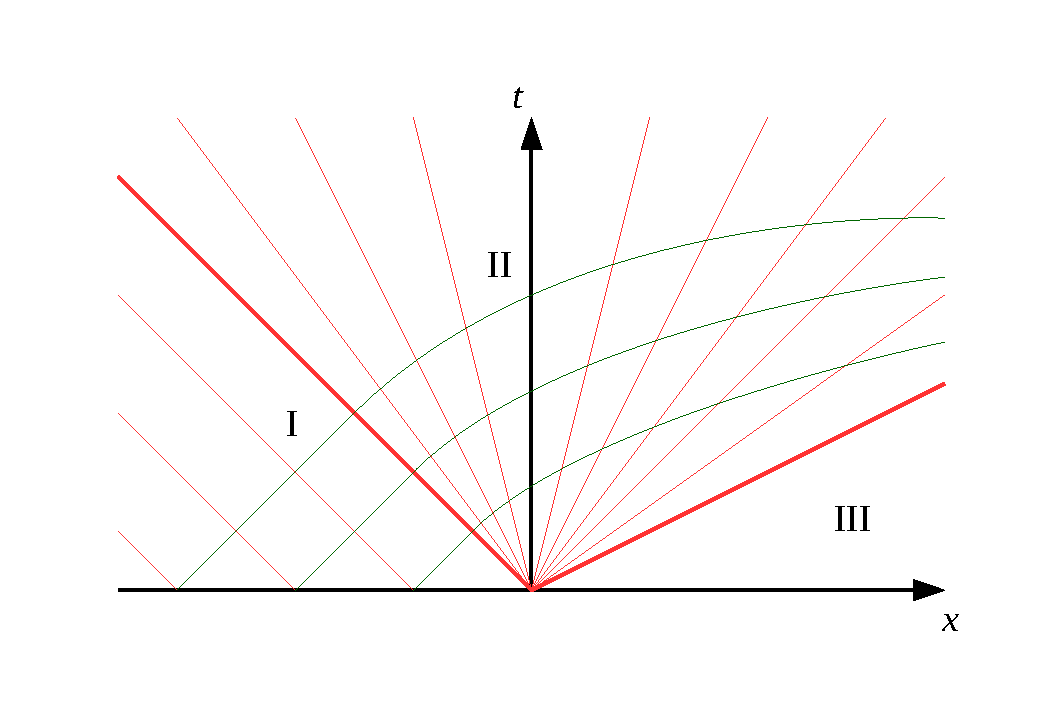
\includegraphics[width=16cm]{st-venant.pdf}
\caption{Characteristics for the St. Venant solution.}
\label{fig:st-venant-chars}
\end{center}
\end{figure}
The characteristics are sketched in Figure \ref{fig:st-venant-chars}.

In Region I, where $x < -c_0 t$, both $C_-$ and $C_+$ characteristics come from the region $x<0$ at $t=0$, and so $u=0$ and $c=c_0$. 

Assume that the $C_+$ characteristics from $x<0$ fill Region II, the region between $x=-c_0 t$ and to the left of the front. (We should check that these characteristics do in fact move faster than the front.) Then $u+2c = 2c_0$ everywhere in that region. But also $u-2c$ is constant along $C_-$ characteristics. Hence $u$ and $c$ must independently be constant along $C_-$ characteristics. Hence $C_-$ characteristics have constant slope $\lambda_- = u - c$. 

If $X_-$ is the position of a $C_-$ characteristic, then 
\begin{equation}
	\dod{X_-}{t} = u-c.
\end{equation}
So $C_-$ characteristics which start at the origin are given by
\begin{equation}
	\frac{x}{t} = u-c.
	\label{st-venant-charposition}
\end{equation}
We solve (\ref{st-venant-charposition}) together with $u+2c=2c_0$ to solve for $u$ and $c$:
\begin{align}
	u &= \frac{2}{3} \left(c_0 + \frac{x}{t}\right) \\
	c &= \frac{1}{3} \left(2c_0 - \frac{x}{t}\right) \\
	h &= \frac{1}{9g} \left(2c_0 - \frac{x}{t}\right)^2.
\end{align}
In particular, $h = 0$ at $x = 2c_0 t$, so the front moves at speed $2c_0$. On the other hand,
\begin{align}
	\lambda_+ &= u+c \\
			&= \frac{4}{3}c_0 + \frac{x}{3t} \\
\end{align}
is the speed at which the $C_+$ characteristics move.

\begin{figure}
\begin{center}
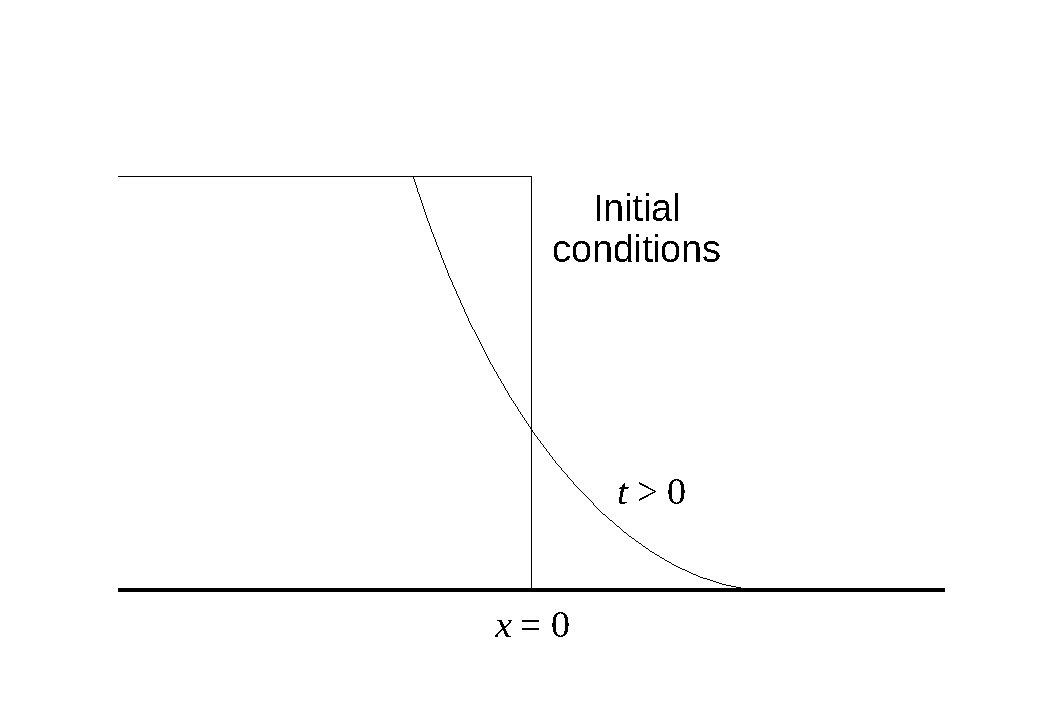
\includegraphics[width=16cm]{st-venant-solution.pdf}
\caption{The St. Venant solution.}
\label{fig:st-venant-solution}
\end{center}
\end{figure}

This is called the St. Venant solution, and it is sketched in Figure \ref{fig:st-venant-solution}. It is not observed in practice. In practice, \textit{bottom drag} and \textit{form drag} have important effects which resist motion. Bottom drag is significant if the current is much more dense than the ambient. Form drag is significant if the ambient is much more dense than the current, or if the density difference is small.

\subsection{Entrainment into shallow water flows}

Turbulent often produces mixing: the blending of fluid particles of a different character. If we have a turbulent shallow water flow, then not only does the turbulence transport momentum within the flow, but it can also drive mixing between the flow and the ambient fluid. In particular, if the turbulence is in the moving shallow water layer, then it can cause the layer to entrain ambient fluid into the layer, affecting its volume, density and possibly its momentum. 

This is true for \textit{miscible fluids}. Immiscible fluids can entrain each other, but the resulting two-phase flow will separate again if allowed to. 

Shallow water flows may be unstable both to short wave instabilities, such as Kelvin-Helmholtz and Holmboe instabilities, and to long wave instabilities. 

Entrainment reduces the density contrast and therefore reduces $g'$. It also increases the volume of the layer of fluid, so increases $h$. For a quiescent ambient, the result of entrainment is that $g'h$ is conserved. Also, the fluid that is being drawn in has a different (zero) momentum. 

\begin{figure}
\begin{center}
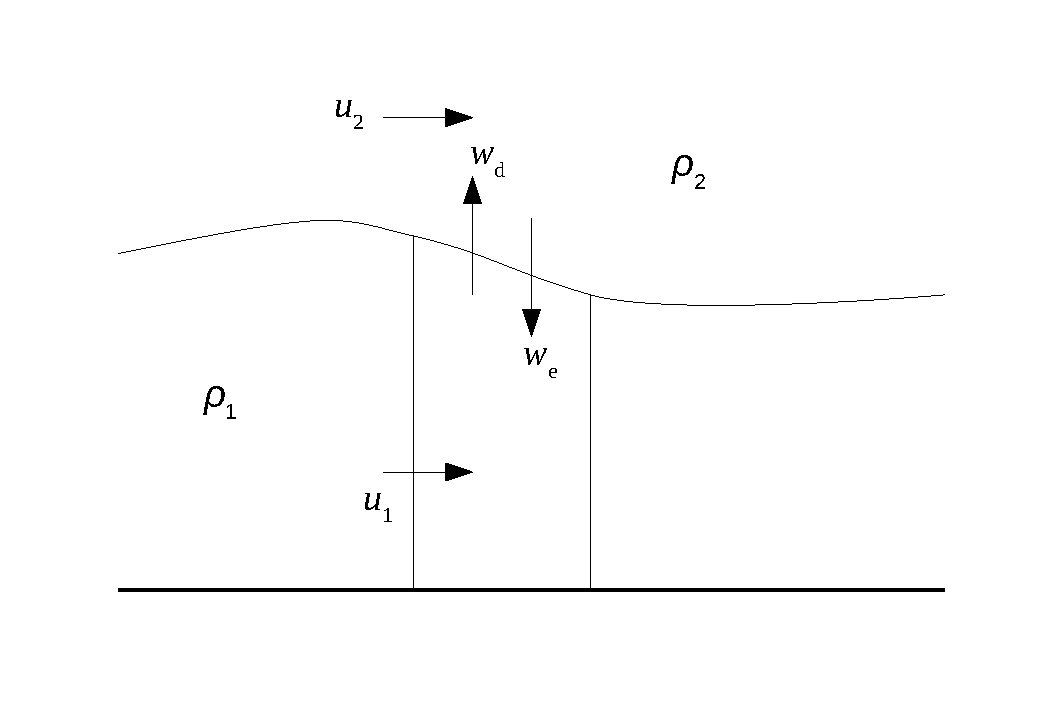
\includegraphics[width=16cm]{entrainment-shallow-water.pdf}
\caption{Schematic for entrainment/detrainment for a shallow layer.}
\label{fig:entrainment-shallow-water}
\end{center}
\end{figure}

The setup is sketched in Figure \ref{fig:entrainment-shallow-water}. Assume that the ambient fluid density $\rho_2$ is constant, so that only the density in the layer $\rho_1$ changes. Let $w_e$ be the speed of entrainment and $w_d$ the speed of `detrainment'. Then, by considering fluxes in and out of a control volume:
\begin{itemize}
	\item Conservation of volume gives
	\begin{equation}
		\dpd{h}{t} + \dpd{}{x} (u_1 h) = w_e - w_d.
	\end{equation}
	\item Conservation of mass gives
	\begin{equation}
		\dpd{}{t} (\rho_1h) + \dpd{}{x} (u_1\rho_1h) = w_e\rho_2 - w_d\rho_1
	\end{equation}
	or, using conservation of volume,
	\begin{equation}
		\dpd{\rho_1}{t} + u_1 \dpd{rho_1}{x} = -\frac{w_e}{h} (\rho_1 - \rho_2)
		\label{swentrain-mass}
	\end{equation}
	\item The momentum balance (ignoring drag) gives
	\begin{equation}
		\dpd{}{t} (\rho_1 hu_1) + \dpd{}{x}\left(
			u_1 \rho_1 hu_1 + \frac{1}{2}(\rho_1 - \rho_2)gh^2 
		\right) = w_e \rho_2 u_2 - w_d \rho_1 u_1.
	\end{equation}
	We get this by taking the pressure to be hydrostatic and equal to $p_0$ at some reference height $z_0$. Then the horizontal pressure gradient, integrated over the horizontal cross section, is 
	\begin{align}
		\int_0^h \dpd{p}{x}\dif z &= \int_0^h \dpd{}{x} (p_0 + \rho_2g(z_0-z) + (\rho_1-\rho_2)g(h-z)) \dif z \\
			&= \cdots \\
			&= \dpd{}{x} \left( \frac{1}{2}g(\rho_1-\rho_2)h^2\right).
	\end{align}
	Using conservation of mass, the momentum equation can also be written as
	\begin{equation}
		\dpd{u_1}{t} + u_1\dpd{u_1}{t} + g \frac{\rho_1-\rho_2}{\rho_1} \dpd{h}{x} + \frac{gh}{2\rho_1}\dpd{}{x}(\rho_1-\rho_2)
		 = -w_e \frac{\rho_2}{\rho_1} \frac{u_1 - u_2}{h}
		 \label{swentrain-mom}
	\end{equation}
\end{itemize}

Note that conservation of volume does not strictly hold: Mass is conserved, but the density of a mixture will be different from the density of its constituents. For `linear mixing', we can ignore changes in volume. We work in the Boussinesq approximation where $\rho_{1,2}$ are approximately equal, and assume that the ambient fluid is stationary: $u_2 = 0$. Then (\ref{swentrain-mom}) reduces to
\begin{equation}
	\dpd{u_1}{t} + u_1\dpd{u_1}{t} + g' \dpd{h}{x} + \frac{h}{2}\dpd{g'}{x}
		 = -w_e \frac{u_1}{h}
\end{equation}
where $g' = g(\rho_1-\rho_2)/\rho$. If we also write (\ref{swentrain-mass}) in terms of $g'$, then 
\begin{alignat}{5}
	\dpd{g'}{t} 		&+ u_1 \dpd{g'}{x}  		&				& 				&= -g'\frac{w_e}{h} \\
	\dpd{h}{t} 		& 					&+ u_1\dpd{h}{x}	&+ h\dpd{u_1}{x} 	&= w_e - w_d \\
	\dpd{u_1}{t} 	&+ \frac{h}{2}\dpd{g'}{x}	&+ g'\dpd{h}{x} 		&+ u_1 \dpd{u_1}{x} 	&= -u_1 \frac{w_e}{h}
\end{alignat}
or, in matrix form,
\begin{equation}
\begin{pmatrix}
 u_1 & 0 & 0 \\
 0 & u_1 & h \\
 \frac{h}{2} & g' & u_1 
\end{pmatrix}
\begin{pmatrix}
g' \\ h \\ u_1
\end{pmatrix} _x + \begin{pmatrix}g'\\h\\u_1\end{pmatrix} _t 
= 
\begin{pmatrix}
 -g'\frac{w_e}{h} \\  w_e - w_d \\  -u_1 \frac{w_e}{h}
\end{pmatrix}.
\label{swentrain-matrix}
\end{equation}

The system is still hyperbolic, as the matrix still admits three real, distinct eigenvalues: $\lambda = u_1$ and $\lambda = u_1 \pm (g'h)^{1/2}$. The latter two represent interfacial waves as before; the characteristic with $\lambda = u_1$ represents the advection of density. Since the RHS of (\ref{swentrain-matrix}) is nonzero, the evolution equations along those characteristics are inhomogeneous:
\begin{itemize}
	\item Along the $\lambda = u_1$ characteristic, we have
	\begin{equation}
		\dpd{g'}{s} = -g' \frac{w_e}/h;
	\end{equation}
	\item along the $\lambda = u_1 + (g'h)^{1/2}$ characteristic,
	\begin{equation}
		\frac{h}{2\sqrt{g'}} \dpd{g'}{s} + \sqrt{g'} \dpd{h}{s} + \sqrt{h} \dpd{u_1}{s}
		 = -\frac{1}{2}\sqrt{g'} w_e + \sqrt{g'} (w_e + w_d) - u_1 \frac{w_e}{\sqrt{h}}.
	\end{equation}
\end{itemize}


\section{Gravity currents}
\subsection{A moving dam problem}
\subsection{Description}
\subsection{Early models}
\subsection{Cavity flows}
\subsection{*Morden and Beiburg}
\subsection{Gravity currents and characteristics}
\subsection{Modelling gravity currents}
\subsection{Real life is more complex}
